\documentclass[12pt,a4paper]{article}
\usepackage[utf8]{inputenc}
\usepackage{amsmath}
\usepackage{amsfonts}
\usepackage[french]{babel}
\usepackage{amssymb}
\usepackage{graphicx}
\usepackage{palatino}
\usepackage{sectsty}
\usepackage[]{listings}
\usepackage{pgfplots}
\usepackage[french, ruled]{algorithm2e}
%\usepackage{fancyhdr}
\usepackage[colorlinks=true,linkcolor=black]{hyperref}
\usepackage{color}
\usepackage[top=3cm, bottom=3cm, left=2.5cm, right=2.5cm]{geometry}
\pagestyle{plain}
\author{Tafsir GNA}

\lstset{frame=lines, numbers=left,numberstyle=\tiny\bfseries\underline, stepnumber=1, firstnumber =1, numberfirstline=true, backgroundcolor={\color[gray]{0.9}}, showstringspaces=false, basicstyle=\rm\footnotesize}


\makeatletter
\renewcommand{\@algocf@capt@plain}{above}% formerly {bottom}
\makeatother

%\allsectionsfont{\sf}
%\sectionfont{\sffamily\color{black}\sectionrule{3ex}{3pt} %
%{-1.5ex}{1pt}}

\begin{document}

\setcounter{section}{0}

	\begin{titlepage}
		\centering
		
		\noindent%
		
		\begin{minipage}{.15\linewidth}
			
\includegraphics[scale=0.4]{img/ifri_logo.png}
		\end{minipage}
		\hfill
		\begin{minipage}{.68\linewidth}\centering
			\textsc{République du Bénin}\\
			\vspace*{.5cm}
			\textsc{\Large Université d'Abomey-Calavi}
		\end{minipage}
		\hfill
		\begin{minipage}{.15\linewidth}
			
\includegraphics[width=1\linewidth]{img/uac_logo.png}
		\end{minipage}
				
		\vspace{1cm}{\scshape\Large Institut de Formation et de Recherche en Informatique (IFRI)\par}
		\vspace{1cm}{\scshape\Large Mémoire pour l'obtention du diplôme de Master en Systèmes d'Information et Réseaux Informatiques\par}
		\vspace{1.5cm}{\huge\bfseries Résolution de "Pigment Sequencing Problem" avec les algorithmes génétiques\par}
		\vspace{2cm}{\scshape \Large\textbf{Présenté par} \\ Tafsir GNA \par}
		\vfill
		\Large\textbf{Supervisé par}\par Pr. Norbert \textsc{Hounkonnou} \\ \& \\ Dr. Ratheil Vinasétan \textsc{Houndji}
		\vfill
		{\large \scshape Année Académique 2016-2017 \par}
	\end{titlepage}

	\newpage % Page de remerciement
	
	\section*{Remerciements}
	\addcontentsline{toc}{section}{Remerciements}	
	
	\vspace{2.5cm}
	
	Je tiens à remercier tous ceux qui ont aidé et participé à la réalisation de ce travail à travers leurs différents apports et soutiens. \\
	\hspace*{.5cm}Je remercie particulièrement : \\
	\begin{itemize}
		\item[•] Pr. Eugène EZIN, Directeur de l'Institut de Formation et de Recherche en Informatique (IFRI) ainsi que tous les membres du corps enseignant et administratif de l'IFRI;
		\item[•] Pr. Norbert HOUNKONNOU, pour avoir accepté de superviser mes travaux ainsi que Dr. Ratheil HOUNDJI pour l'encadrement et les conseils apportés;
		\item[•] Mon père, ma mère et par extension toute ma famille pour leur soutien et leurs encouragements. 
	\end{itemize}
	
	\newpage
	% Tables des matières
	\tableofcontents
	
	\newpage
	
	%Liste des figures
	\listoffigures
	\addcontentsline{toc}{section}{Liste des figures}
	
	\newpage
	
	%Liste des Tableaux
	\listoftables
	\addcontentsline{toc}{section}{Liste des tableaux}
	
	\newpage
	
	%Liste des algorithmes
	\listofalgorithms
	\addcontentsline{toc}{section}{Liste des algorithmes}
	
	\newpage
	\section*{Glossaire:}
	\addcontentsline{toc}{section}{Glossaire}	
	
	\vspace{1cm}
	
	\textbf{PSP} : Pigment Sequencing Problem \\
	\hspace*{.5cm} \textbf{AG} : Algorithme Génétique \\
	\hspace*{.5cm} \textbf{F-PGA} : Fine-grained Parallel Genetic Algorithm \\
	\hspace*{.5cm} \textbf{C-PGA} : Coarse-grained Parallel Genetic Algorithm \\
	\hspace*{.5cm} \textbf{CLSP} : Capacited Lot Sizing Problem \\
	\hspace*{.5cm} \textbf{DFS} : Depth First Search
	
	
	\newpage % Page du résumé en français
	
	\section*{Résumé:}
	\addcontentsline{toc}{section}{Résumé}	
	
	\vspace{1cm}
	
	Le dimensionnement de lot est la tâche la plus difficile et la plus importante dans les problèmes de planification de production en industrie. Il consiste à identifier, sur un horizon de planification, le nombre (et le type) d’articles à produire et à quel moment produire de façon à minimiser le coût total de production. De récentes recherches ont expérimenté une variante NP-Difficile du problème de dimensionnement de lot : le “Pigment Sequencing Problem” (PSP). Aussi, les algorithmes génétiques ont montré leur efficacité sur des problèmes d’optimisation difficiles en trouvant de relativement bonnes solutions par rapport aux solutions optimales. Ce travail vise à donc travers l'application deux méthodes de recherche basées sur les algorithmes génétiques au “Pigment Sequencing Problem”, à identifier un plan de production qui respecte les capacités de production des machines tout en minimisant les coûts de stockage et de transition d’une production à une autre. \\
	\\
	\hspace*{.5cm}\textsl{\textbf{Mots clés :}} Algorithme génétique, planification de production, pigment sequencing problem, dimensionnement de lot.
	
	\newpage % Page du résumé en anglais
	
	\section*{Abstract:}
	\addcontentsline{toc}{section}{Abstract}
	
	\vspace{1cm}
	
	The lot sizing is the most difficult and important task in production planning problems in industry field. It involves determining through a planning horizon the number (and the type) of the items to manufacture and when to manufacture these items in order to minimize the overall cost of manufacturing. Some recent researches have experienced a NP-hard variant of lot sizing problem called "Pigment Sequencing Problem" (PSP). Besides, Genetic Algorithms (GA) have shown how effecient they are, in finding some relatively good solutions in comparison to the optimal ones. Thus, This work aims to apply two heuristic approaches based on genetic algorithms to the Pigment Sequencing Problem, to find a solution that fits into the machine capacity restrictions and that minimizes the stocking costs and change-over costs from one item to another one.\\
	\\
	\hspace*{.5cm}\textsl{\textbf{Key words :}} Genetic algorithm, production planning, pigment sequencing problem, lot sizing.
	
	  
	
	\newpage
	
	\part*{Introduction}
	\addcontentsline{toc}{part}{Introduction}
	
	Dans un processus de planification de production, le dimensionnement
de lots (lot sizing) qui consiste à identifier les articles à produire, quand il
faut les produire et sur quelle machine de façon à satisfaire les demandes
tout en considérant les objectifs financiers, est l’activité la plus importante
et la plus difficile. En effet, de la qualité des décisions qui seront prises
dépendent la performance et la compétitivité de l’entreprise. Connu dans la
littérature sous le nom de problème de lot sizing, il a été beaucoup étudié
ces dernières décennies depuis les travaux de Wagner et Within en 1958. \\
	\hspace*{.5cm} Différentes versions de dimensionnement de lots ont été proposées dans le littérature, chacune étant spécifique à leur domaine d'application. Récemment, (Houndji et al., “The stockingCost constraint”, 2014) et (Ceschia et al., opthub.uniud.it, 2016) ont expérimenté une variante NP-Difficile du problème de dimensionnement de lots. Cette version est connue comme le “Pigment Sequencing Problem” (Pochet et Wolsey 2006, §14.4) et a été récemment inclue à la bibliothèque CSPlib (Gent and Walsh, 1999, prob058) . Il s'agit de produire plusieurs articles avec une seule machine dont la capacité de production est limitée à un article par période. L'horizon de planification est discret et fini, et il y a des coûts de stockage et des coûts de transition d'une production à une autre. Par ailleurs, les demandes sont normalisées et donc binaires. \\
	\hspace*{.5cm} Dans la plupart des cas, un problème d’optimisation tel que le problème de dimensionnement de lots se divise naturellement en deux phases : recherche des solutions admissibles puis recherche de la solution à coût optimal parmi ces dernières. Suivant la méthode employée, ce découpage est plus ou moins apparent dans la résolution. L’usage d’un algorithme génétique est adapté à une exploration rapide et globale d’un espace de recherche de taille importante et est capable de fournir plusieurs solutions. Des calculs effectués ont révélé que l'utilisation des algorithmes génétiques pour des problèmes de dimensionnement de lots semble raisonnable dans le cas de grands problèmes où trouver la solution avec d'autres algorithmes reste encore problématique en temps. Ainsi, Il est possible qu'un algorithme génétique convenablement construit et paramétré puisse trouver de bien meilleurs résultats comparativement à ceux trouvés par d'autres algorithmes tels que le programmation en nombre entier et cela pour un même laps de temps considéré.
	
	\section*{Notre contribution}
	Le "Pigment Sequencing Problem" est un problème NP-Difficile d'optimisation combinatoire pour lequel les instances de taille moyenne peuvent être efficacement résolues en utilisant une formulation appropriée de programmation en nombre mixte. Cependant, dans notre revue de littérature, aucun modèle basé sur les algorithmes génétiques n'a encore été proposé pour ce problème. Nous proposons donc deux méthodes basées sur les algorithmes génétiques pour le problème. La première est une méthode appelée "coarse-grained parallel genetic algorithm" qui divise la population globale en sous-populations. La seconde, appelée "fine-grained parallel genetic algorithm" qui réduit le champ de crossover à l'environnement immédiat. Les tests que nous avons menés afin de valider nos deux méthodes ont produit des résultats satisfaisants et confirmé le fait que les algorithmes génétiques sont efficaces quant il s'agit de résoudre des problèmes d'optimisation. 
	 
	\section*{Organisation du travail}

	Le travail effectué est organisé dans ce document en 4 parties. Le première partie présente une revue de littérature des problèmes de dimensionnement de lots en planification de production en nous concentrant sur les classes de problèmes qui nous concerne particulièrement. Nous présentons également dans cette partie les algorithmes génétiques, leurs étapes ainsi que leurs fonctionnement. Dans le deuxième partie, nous présentons dans un premier temps, les modèles mathématiques spécifiques au PSP ainsi que leur formulation, utilisés afin de résoudre le PSP. En troisième partie, nous détaillons les deux méthodes de recherche utilisés dans leurs différents aspects ainsi que les algorithmes utilisés. Ensuite, en dernière et quatrième partie, nous expérimentons  nos deux méthodes, présentons les résultats obtenus et comparons ces résultats à l'état de l'art en la matière. Pour finir, nous tirons une conclusion du travail effectué et dressons les perspectives possibles en vue d'améliorer ce qui a été fait.
	
	\newpage
	
	\part{Etat de l'art}
	%\newpage
		\section*{Introduction}
		\addcontentsline{toc}{section}{Introduction}
		L'état de l'art revêt une grande importance dans la conduite d'un travail de recherche. Elle permet de fixer les idées quant au travail qui a été déjà fait dans le domaine. Il s'agira donc principalement dans cette première partie de présenter la revue de littérature des problèmes de dimensionnement de lot en planification de production, d'exposer les travaux sur les algorithmes génétiques et de montrer en quoi les algorithmes génétiques sont particulièrement adaptés à ces genres de problèmes.
		
	\section{Le dimensionnement de lot en planification de production}
	La planification de production est un processus qui consiste à déterminer un plan qui indique quelle quantité d'articles produire durant un intervalle de temps appelé "horizon de planification". Il est un important défi pour les entreprises industrielles car il a un fort impact sur leur performance en terme de qualité du service-client et des coûts d'exploitation.	
	
	\subsection{Problématique}
		
 La planification de production s'avère être une tâche très complexe principalement pour les raisons suivantes:
 \begin{itemize}
 	\item[-] Le plus souvent, une ressource de production n'est pas seulement dédiée à un unique article, mais plutôt utilisée pour produire différents types d'articles. Dans un contexte de processus d'industrie, les ressources de production disponibles ne pas vraiment flexibles et ne peuvent produire qu'un type d'article à la fois. En conséquence, la planification de production se heurte à la compétition entre les articles partageant les mêmes ressources et il faut décider quels articles produire, quand et en quelle quantité, tout en prenant en compte les contraintes liées au système de production. Dans certains cas, ces contraintes peuvent être si rigides que trouver une plan de production valide et faisable peut être difficile.
 	
 	\item[-] Un plan de production doit remplir plusieurs objectifs souvent contradictoires, notamment, garantir un excellent niveau du service-client et minimiser la production et les coûts de stockage. Ainsi, les mesures basiques telles que, ne pas satisfaire la demande excédant les capacités de production et garder une haut niveau de stockage afin d'être capable de répondre à toute demande ne sont pas commercialement acceptables ou encore trop chères. Un bon plan de planification est donc le résultat d'un compromis entre différents objectifs contradictoires.
 	\item[-] Un plan de production n'est jamais fixé pour toujours. Sa validité est restreinte à un horizon de planification prédéfini. De plus, la réalité dévie le plus souvent des prévisions et si la divergence entre les plans et les prévisions est trop grande, le plan doit être revu avant la fin de l'horizon de planification.
 \end{itemize}
 
 La planification de production est donc un problème difficile et récurrent pour les compagnies industrielles. Il y a un fort besoin de systèmes d'aide à la décision. Le développement de tels systèmes a été l'objectif d'une grande partie de la littérature en recherche opérationnelle pour les cinquante dernières années. 
	
\subsection{Critères de classification}

Différents critères interviennent dans la classification des problèmes de dimensionnement de lot, notamment : 
\begin{description}
	\item[\textsl{L'échelle de temps}:] La planification peut être effectuée soit sur des périodes discrètes soit sur un
horizon de temps continu. Dans le premier cas, la longueur des périodes peut
être soit de petite taille (Small time buckets) correspondant à des heures ou
jours, soit de grande taille (Big time buckets) correspondant à des jours ou
semaines, soit de très grande taille (Very big time buckets) correspondant à
des mois ou trimestres.

	\item[\textsl{Le nombre de niveaux}:] Dans le cas où seules les demandes venant de l'extérieur du système sont considérées, on parle de problèmes à un niveau. Un état de l'art sur ce type de problème est proposé par Karimi et al. [71]. Lorsqu'il existe une relation entre
les produits, on considère des problèmes à plusieurs niveaux. Ce dernier type
de problèmes se retrouve fréquemment dans l'industrie.

	\item[\textsl{Le nombre de produits}:] Dans le cas où il n'y a pas de dépendance entre les produits, en particulier, s'il n'y a pas d'utilisation commune de la capacité, nous considérons des problèmes
à un seul produit. Dans le cas inverse, on parle de problèmes à plusieurs produits. Un état de l'art sur les problèmes à un produit est proposé par Brahimi
et al. [16].

	\item[\textsl{Les contraintes de capacité}:] Les contraintes de capacité incluent le nombre d'employés, la capacité des machines, la capacité de stockage, etc. Lorsque les contraintes de capacité sont
introduites dans le modèle, elles rendent le problème plus difficile à résoudre,
puisqu'elles lient les produits entre eux.

	\item[\textsl{Les demandes}:] Il existe plusieurs types de demandes qui peuvent être réparties selon trois
groupes :
	\begin{itemize}
		\item[•] Demandes constantes , les valeurs des demandes ne changent pas sur l'horizon de temps, ou demandes dynamiques , les valeurs varient au cours du temps.
		\item[•] Demandes certaines , les valeurs sont connues à l'avance, ou demandes stochastiques , les valeurs sont basées sur des probabilités.
		\item[•] Demandes indépendantes , lorsqu'un produit n'a pas besoin d'autres produits comme composants, ou demandes dépendantes , lorsqu'il existe une relation
entre les produits.
	\end{itemize}

	\item[\textsl{Les coûts et temps de lancement ou préparation (setup)}:] Une ressource peut exécuter des produits de types différents. Ainsi, il est parfois nécessaire de reconfigurer celle-ci à chaque changement de produits. Les coûts et temps induits par le lancement de la ressource sont souvent importants car
élevés et longs.
	
\end{description}

	La complexité des problèmes de dimensionnement de lots varie fortement sous l'influence des différents facteurs comme le nombre de produits, le nombre de niveaux, les contraintes de capacité, etc. Nous avons choisi dans cette étude de décrire les problèmes de dimensionnement de lots selon la longueur de la période de l'horizon de temps. Nous allons donc nous intéresser aux problèmes à courtes et longues périodes.
\subsection{Classes}
	\subsubsection{Problèmes à courtes périodes}
	Ces problèmes (\emph{Small time bucket problems}) sont caractérisés par des périodes de l'ordre de quelques heures, et la séquence des lots lors de la production est prise en compte. Quatre types de problèmes sont étudiés dans la littérature. Pour une étude détaillée de tous ces problèmes, nous pourrons nous référer à Drexl and Kimms [35]. Ces différents types de problèmes sont donc:
	\begin{description}
		\item[\textsl{Discrete lot-sizing and scheduling problem :}]
		Ce problème noté DLSP, est initialement formulé par Fleischmann [43]. La principale hypothèse de ce problème est qu'au plus un article peut être produit par
période. Si un article est fabriqué sur une période, alors toute la capacité disponible sur cette période sera utilisée. Généralement, les coûts de lancement sont pris en compte seulement lorsqu'un nouveau lot commence et non à chaque période.
		\item[\textsl{Continuous setup lot-sizing problem :}]
		Ce problème noté CSLP est similaire au précédent problème. La différence réside dans le fait que lorsqu'un article est produit sur une période, on utilise la capacité nécessaire pour produire cet article et non la capacité entière comme pour le problème précèdent.
		\item[\textsl{Proportional lot-sizing and scheduling problem : }] 
		Dans ce problème, que l'on notera PSLP, la capacité restante pour une période donnée est réutilisée pour produire un second article. Ce problème a été étudié par Drexl et Haase [34] et Kimms et Drexl [78]. Il existe des extensions pour ce problème, par exemple, le cas à plusieurs niveaux et plusieurs machines. Dans [76], Kimms propose de calculer des bornes inférieures, et il résout ce problème à l'aide d'un algorithme génétique dans [77].
		\item[\textsl{General lot-sizing and scheduling problem : }] 
		Ce problème noté GLSP, est plus général que les problèmes précédents, puisque le nombre d'articles à produire par période n'est pas restrictif. Il est étudié par Fleischmann et Meyr [44]. Il existe des extensions de ce problème, par exemple en intégrant des temps de lancement de production dépendant de la séquence des lots à produire ([93]).
	\end{description}
	
	\subsubsection{Problèmes à longues périodes}
	Les problèmes à longues périodes (\emph{Big time bucket problems}) sont basés sur des
horizons de l'ordre de quelques jours à quelques semaines et sont caractérisés par le fait que plus d'un produit peut être fabriqué par période. Nous proposons dans cette section, une étude restreinte de ces problèmes.
	
	\begin{description}
		\item[Les problèmes à un niveau et un produit]: \\
		Ces problèmes ne correspondent pas vraiment à la réalité mais reçoivent beaucoup d'attention et d'intérêt puisque les méthodes mises en œuvre pour les résoudre sont généralisées dans le cas des problématiques à plusieurs niveaux.
		Les premiers travaux sur cette problématique ont été conduits par Manne [90]
et Wagner et Whitin [129]. Leur méthode de résolution est utilisée dans plusieurs
concepts pour résoudre des problèmes plus complexes. Brahimi et al. [16] ont proposé
un état de l'art sur ces problématiques.		
		\item[Les problèmes à un niveau et plusieurs produits]: \\
		Le problème de dimensionnement de lots avec contraintes de capacité est considéré comme un problème complexe puisque la contrainte de capacité engendre un
lien entre les différents produits. Dans le cas où la capacité est considérée comme
infinie, le problème de dimensionnement de lots à N produits est réductible à N
problèmes à un produit et sans capacité, chacun solvable en temps polynomial.
		\item[Les problèmes à plusieurs niveaux]: \\ 
		Ces problèmes sont caractérisés par le fait que les produits finis sont fabriqués à partir de produits intermédiaires. Ainsi, les demandes dépendantes (i.e. les demandes entre les produits) et les demandes indépendantes (i.e. les demandes arrivant de l'extérieur) sont prises en compte dans ce type de problème.
	\end{description}
	
	Un exemple typique d'un problème de "\emph{big bucket}" est le "Capacited Lot Sizing Problem" (CLSP) , où différents articles peuvent être produit sur une même ressource en une seule période. Le CLSP classique consiste à déterminer le coût et le temps de production des articles dans l'horizon de planification: le résultat est un plan de production qui donne pour chaque période de planification, la quantité (\emph{lot size}) de chaque article qui doivent être produit. Le CLSP requiert que la ressource soit préparée pour un article donné dans la période où il est produit. 
	
	\begin{center}
		\begin{figure}[!h]
			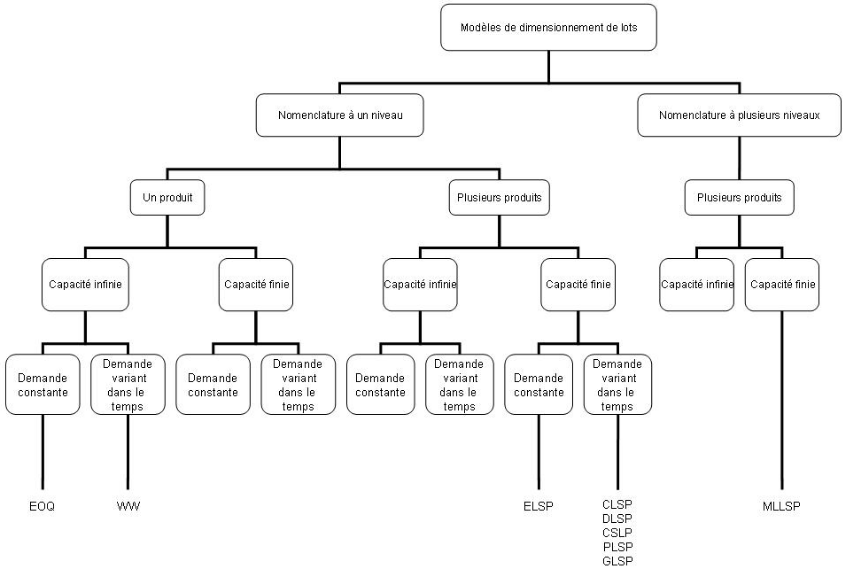
\includegraphics[scale=.5]{img/classification_dimensionnement.png}
			\caption{Exemple de classification des modèles de dimensionnement de lots}
		\end{figure}
	\end{center}

	\newpage
	
	\section{Les algorithmes génétiques}
	Les algorithmes génétiques (AGs) sont des algorithmes d’exploration fondés sur les mécanismes de la sélection naturelle et de la génétique. Ils utilisent à la fois les principes de la survie des structures les mieux adaptées, et les échanges d’informations aléatoires, parfois guidés, pour former un algorithme d’exploration qui possède certaines des caractéristiques de l’exploration humaine. Ils ont été développés par John Holland [7] à l’université du Michigan.
	\subsection{Concepts de base}
	Les AGs constituent une classe de stratégies de recherche réalisant un compromis entre l’exploration et l’exploitation. Ils représentent des méthodes qui utilisent
un choix aléatoire comme outil pour guider une exploration intelligente dans l’espace des paramètres codés. Ce sont des algorithmes itératifs de recherche globale dont l’objectif est d’optimiser une fonction prédéfinie appelée fonction coût ou fonction « fitness » f.
	Les algorithmes génétiques emploient un vocabulaire emprunté à la génétique naturelle. Ils travaillent sur un ensemble d’individus appelé population. Un individu a deux représentations appelées phénotype et génotype. Le phénotype représente une solution potentielle du problème à optimiser en utilisant la formulation originale du problème. Le génotype donne une représentation codée
d’une solution potentielle sous la forme d’un chromosome. Un chromosome est formé de gènes disposés en une succession linéaire et chaque gène peut prendre plusieurs
valeurs appelées allèles. Par exemple, un chromosome se compose d’une succession de 0 et de 1 (c.-à-d. une chaîne binaire), et la valeur pour une certaine position correspond à on (la valeur = 1) ou à off (la valeur = 0) d’un certain dispositif. Des formes plus compliquées, telles qu’un ordre des symboles et une permutation des alphabets, sont choisies pour décrire les chromosomes du problème à optimiser. Chaque individu a une fonction objectif f (fonction « fitness ») qui mesure l’adaptation de l’individu à son environnement local. La théorie darwinienne indique que, parmi des individus d’une population, celui qui est le mieux adapté à l’environnement local a le plus de chance de survivre et d’avoir un plus grand nombre de descendants : c’est la règle de la « survie du plus fort ». Ainsi, la
fonction objectif f du problème d’optimisation joue le rôle d’un critère d’adaptation [18]. Un des points les plus importants des algorithmes génétiques est la flexibilité dans la fonction objectif.

	\subsection{Fonctionnement}
	
	Le principe de fonctionnement de l'algorithme génétique simple est représenté comme suit: \\
	 
	\begin{algorithm}[H]
 	\caption{Algorithme génétique standard}
 	%\KwData{this text}
 	%\KwResult{how to write algorithm with \LaTeX2e }
 	%initialization\;
 	Générer la population initiale Pi \\
 	Évaluer la population Pi \\
 	\While{le critère de terminaison n'est pas satisfait}{
 	 Sélectionner les éléments de Pi à copier dans P i+1 \\
 	 Appliquer le crossover aux éléments de Pi et les mettre dans P i+1 \\
 	 Appliquer la mutation aux éléments de Pi et les mettre dans P i+1 \\
 	 Évaluer la nouvelle population P i+1 \\
 	 Pi = P i+1
 	}
	\end{algorithm}
	
	\vspace*{1cm}
	Cet algorithme est explicité plus en détails à l'aide de la figure suivante.
	
	\begin{figure}[!h]
		\begin{center}
			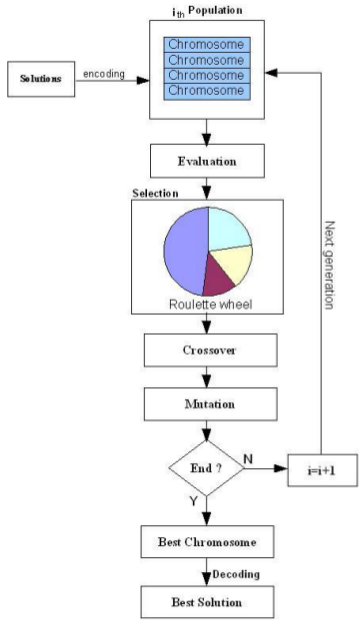
\includegraphics[scale=.5]{img/genetic_algo_flowchart.png}
			\caption{Diagramme d'un algorithme génétique standard}
		\end{center}
	\end{figure}
	
	\newpage
	
	\subsection{Les opérateurs}
		Un algorithme génétique simple utilise les trois opérateurs suivants : la sélection, le croisement et la mutation.
		\subsubsection{L’opérateur de sélection}
		La sélection est un processus dans lequel des individus d’une population sont choisis selon les valeurs de leur fonction coût ou «  fitness  » pour former une nouvelle population. Les individus évoluent par des itérations successives de la sélection, appelées générations. Chaque individu est sélectionné proportionnellement à sa fonction « fitness », donc, un individu avec une fonction « fitness »
plus élevée aura plus de chance d’être sélectionné qu’un autre avec une valeur de « fitness » inférieure. Cette fonction peut être envisagée comme une mesure de profit ou de qualité qu’on souhaite maximiser. Un opérateur simple de sélection est la technique de la roulette pondérée où chaque individu d’une population
occupe une surface de la roulette proportionnelle à la valeur de sa fonction « fitness ». Pour la reproduction, les candidats sont sélectionnés avec une probabilité proportionnelle à leur «  fitness  ». Pour chaque sélection d’un
individu, une simple rotation de la roue donne le candidat sélectionné. Cependant cette sélection n’est pas parfaite. En effet, le risque de favoriser un individu ou un petit ensemble d’individus constitue un inconvénient qui risque d’appauvrir la diversité de la population.
	\subsubsection{L’opérateur de croisement}
	Le croisement est un opérateur de recombinaison. Les individus d’une population sont couplés au hasard par paires représentant les parents. Chaque paire d’individus
subit le croisement décrit comme suit : le croisement opère sur les génotypes (c.-à-d. les chromosomes) de deux individus appelés parents. Il produit de nouveaux individus (généralement deux) appelés enfants dont les gènes sont hérités de l’un ou/et de l’autre parent. Ceci peut être fait en dédoublant chacun des deux chromosomes dans des fragments et en les recombinant pour former de nouveaux chromosomes.
	\begin{description}
		\item[\textsl{Le croisement à un point :}] Si le génotype est une chaîne binaire de longueur n. Le croisement à un point place un point de croisement au
hasard. Un enfant prend une section avant le point de croisement d’un parent et prend l’autre section après le point de croisement de l’autre parent puis recombine les deux sections pour former une nouvelle chaîne binaire. L’autre enfant se construit inversement. Exemple : considérons P1 et P2 deux chaînes binaires de
longueur n = 7 comme parents :
	\begin{center}
		P1 = 0 0 0 0 | 0 0 1 \\
		P2 = 1 1 1 1 | 1 1 0
	\end{center}
	\hspace*{.5cm} Le symbole | indique un point de croisement, dans cet exemple il est placé après le quatrième bit. \\
	\hspace*{.5cm} Le croisement à un point crée les deux nouveaux individus E1 et E2 comme suit :
	\begin{center}
		E1 = 0 0 0 0 | 1 1 0 \\
		E2 = 1 1 1 1 | 0 0 1
	\end{center}
		
		\item[\textsl{Le croisement à deux points :}]Le croisement à deux points place deux points de croisement au hasard, et prend une section entre les points d’un parent et les autres sections en dehors des points de l’autre parent puis les recombine. Dans l’exemple suivant, les deux points de croisement sont placés respectivement après le premier et quatrième bit :
	
	\begin{center}
		P1 = 0 | 0 0 0 | 0 0 1 \\
		P2 = 1 | 1 1 1 | 1 1 0
	\end{center}
	
	Le croisement à deux points résultant rapporte les deux individus suivants :
	\begin{center}
		E1 = 0 | 1 1 1 | 0 0 1 \\
		E2 = 1 | 0 0 0 | 1 1 0
	\end{center}
	
		\item[\textsl{Le croisement uniforme :}]Ce type de croisement a été proposé par Syswerda [14]. Il consiste à choisir avec la même probabilité un allèle de l’un ou de l’autre parent, pour transmettre sa valeur à la même position, aux enfants. Comme le montre l'exemple suivant:
	\begin{center}
		P1 = 0 0 0 0 0 0 1 \\
		P2 = 1 1 1 1 1 1 0 \\
		M = 1 1 0 1 0 0 1
	\end{center}
	
	\begin{center}
		E1 = 0 0 1 0 1 1 1 \\
		E2 = 1 1 0 1 0 0 0
	\end{center}
	
	M représente le masque de transmission dont le principe est le suivant : si la valeur dans le masque est égale à 1, alors la valeur de l’allèle du parent 1 passe à l’enfant 1 (respectivement du parent 2 passe à l’enfant 2) ; sinon la valeur de l’allèle du parent 1 passe à l’enfant 2 (respectivement du parent 2 passe à l’enfant 1), tout en respectant la même position de l’allèle.
	\end{description}
	
	\subsubsection{L'opérateur de mutation}
	
	La mutation opère sur le génotype d’un seul individu. Elle correspond, dans la nature, à une « erreur » qui se produit quand le chromosome est copié et reproduit. Dans une approche numérique, pour une chaîne binaire, elle consiste par exemple à faire pour un allèle un échange entre le « 0 » et le « 1 ». Si des copies exactes sont toujours garanties, alors le taux de mutation est égal à zéro. Cependant, dans la vie réelle, l’erreur de copie peut se produire dans diverses circonstances comme sous l’influence d’un bruit. La mutation change les valeurs de certains gènes avec une faible probabilité. Elle n’améliore pas, en général, les solutions, mais elle évite une perte irréparable de la diversité.
	\begin{center}
		A = 1 0 0 0 0 (avant mutation) \\
		A' = 1 0 1 0 0 (après mutation)
	\end{center}
	
	\subsection{Application des algorithmes génétiques aux problèmes d'optimisation}
	
	Cette approche a été largement utilisée ces dernières années [9, 12, etc.]. L’utilisation des AGs dans de nombreux domaines a fait ses preuves, notamment dans des problèmes combinatoires tels que les problèmes d’ordonnancement [4, 13, 18, 5] et les problèmes de collecte et de distribution. Les problèmes d’ordonnancement d’un atelier classique de type Job-Shop (JSP) ont notamment été largement étudiés et résolus par les AGs [1, 3, 6, 10, 11, 15, etc.]. D’autres algorithmes hybrides ont été aussi proposés [2, 8, 16]. La difficulté principale dans la résolution de ces types de problèmes résulte dans la façon avec laquelle ils sont représentés sous forme algorithmique. Cette phase, la définition du chromosome, représente le point le plus important dans la recherche génétique. Plusieurs approches de représentation
et différents types d’opérateurs d’AGs ont été proposés, pour résoudre ces problèmes.
	
	\section*{Conclusion}
	\addcontentsline{toc}{section}{Conclusion}
	Le dimensionnement de lots en planification de production est un important défi pour les entreprises industrielles. Il consiste à trouver un plan de production qui satisfait aux contraintes spécifiques relatives au système de production. Plusieurs méthodes peuvent servir à résoudre ce problème. Au nombre de ces problèmes, figurent les algorithmes génétiques. Les AGs, à travers l'exploration et l'exploitation de l'espace de recherche ont permis de résoudre bon nombre de problèmes d'optimisation par le passé. Nous présentons dans la partie suivante le PSP ainsi que les modèles et leur formulation qui ont été utilisés dans sa résolution.
		
	\newpage
	
	\part{Description et Modèles du Pigment Sequencing Problem}
	\label{part:psp}
	
	\setcounter{section}{0}
	
	%\newpage
		\section*{Introduction}
		\addcontentsline{toc}{section}{Introduction}
		L'étude des problèmes de dimensionnement de lots au cours de décennies de recherche a permis de développer différents modèles et formulations correspondant à différents problèmes spécifiques. L'étude du "Pigment Sequencing Problem" (PSP) n'échappe pas à la règle. Dans ce chapitre, nous présentons dans un premier temps une description de PSP. Puis dans un second temps, nous détaillons les différents modèles mathématiques utilisées afin de représenter et résoudre le problème.
		
		\section{Description du problème}
		\label{sec:problem_description}
		Le PSP consiste à trouver un plan de production
de plusieurs articles à partir d’une machine avec des côuts de changeover . Les
coûts de changeover sont les coûts encourus lors du passage de la production
de l’article i à celui de l’article j avec $i \neq j$. Le plan de production doit
satisfaire les demandes des clients tout en :
	\begin{itemize}
		\item[•] respectant la capacité de production de la machine;
		\item[•] minimisant les coûts de stockage et de changeover.
	\end{itemize}
	\hspace*{.5cm} On suppose que la période de production est suffisamment courte pour ne produire qu’au plus un article par période et que les demandes sont normalisées : la capacité de production de la machine est limitée à un article par
période et d(i, t) $ \in $ {0, 1} avec i l’article et t la période.\\
	\hspace*{.5cm} Il s’agit d’un problème de planification de production ayant les caractéristiques suivantes : un horizon de planification discret et fini ; des contraintes de capacité ; une demande statique et déterministe ; multi-item et small bucket, des coûts de changeover; un seul niveau; sans shortage.\\

	\textbf{\textsl{Illustration}} : Soit un problème avec les données ci-dessous : \\
	\begin{itemize}
		\item[•] Nombre d’articles : $NI = 2$;
		\item[•] Nombre de périodes : $NT = 5$;
		\item[•] Demande par période. Soit d(i, t) la demande de l’article i à la période t : $d(1, t) = (0, 1, 0, 0, 1)$ et $d(2, t) = (1, 0, 0, 0, 1)$;
		\item[•] Coût de stockage. Soit h(i) le coût de stockage de l’article i : $h(1) = h(2) = 2$;
	\end{itemize}
	Soit \emph{xT} le plan de production qui représente une solution potentielle du problème. Il s’agit d’un tableau de dimension \emph{NT} , contenant à son indice t (avec $t  \in  {1...NT}$) l’article i à produire. Une solution admissible du problème est : $ xT = (2, 1, 2, 0, 1)$ avec un coût de $ q(2, 1) + q(1, 2) + q(2, 1) + 2 * h(2) = 15 $. La solution optimale est : $ xT = (2, 1, 0, 1, 2)$ avec un coût de $q(2, 1) + q(1, 2) + h(1) = 10$.
		
		\section{Modèles et formulations}
		Différents modèles ont été proposés afin de représenter les problèmes de planification de production. Suivant le niveau du problème (single-level ou multi-level), le nombre de ressources à considérer (single-resource ou multi-resource) ou que le problème soit encore \emph{small bucket} ou \emph{big bucket}, les modèles en planification de production se rangent dans différentes catégories.   Dans les modèles \emph{small bucket}, au plus un type d'article  peut être produit sur une ressource durant chaque période de temps. Ainsi, un unique article est affecté à chaque période de planification et la séquence d'affectation article-période qui en résulte, définit le plan de production. Aussi dans les modèles \emph{small bucket}, la production d'un lot peut s'étaler sur plusieurs périodes et les coûts de production ne sont pris en compte que s'il y a un nouveau lot à produire. Pour modéliser cela, de nouvelles variables encore appelées variables de \emph{setup} ou variables de \emph{change-over} dans le cas du PSP sont utilisées. \\
		\hspace*{.5cm} Ainsi, le modèle suivant proposé par Pochet et Wolsey (2006, §14.4) s'avère à la fois intéressant et satisfaisant dans le cadre de notre étude.\\
		\\
		\subsection{Modèle MILP 1}
		\subsection{Modèle MILP 2}
		\subsection{Modèle MILP 3}
		\textbf{\textsl{Modèle utilisé}} :
		\begin{eqnarray}
			min \sum_{i,j,t} q^{i,j}ch_{t}^{i,j} + \sum_{i,t} h^{i} s_{t}^{i} \\
			s_{0}^{i} = 0, \forall i \\
			x_{t}^{i} + s_{t-1}^{i} = d_{t}^{i} + s_{t}^{i}, \forall i,t \\
			x_{t}^{i} \leq y_{t}^{i}, \forall i,t \\
			\sum_{i} y_{t}^{i} = 1 , \forall t \\
			ch_{t}^{i,j} = y_{t-1}^{i} + y_{t}^{j} - 1, \forall i,j,t \\
			x,y,ch \in \{0,1\}, s \in N, i \in \{0..NI\}, t \in \{1..NT\}
		\end{eqnarray}
		
		avec les variables de décisions suivantes: \\
		\begin{itemize}
			\item[-] $x_{t}^{i}$ : variable binaire de production qui vaut 1 si l’article i est produit à la période t et 0 sinon ;
			\item[-] $y_{t}^{i}$ : variable binaire de setup qui vaut 1 si la machine est préparée pour la production de l’article i et 0 sinon ;
			\item[-] $s_{t}^{i}$ : variable entière de stockage qui contient le nombre d’articles i stockés à la période t ; 
			\item[-] $ch_{t}^{i,j}$ : variable binaire de changeover qui vaut 1 si à la période t, on est passé de la production de l’article i à l’article j et 0 sinon.
		\end{itemize}
		\vspace*{.3cm}
		\textbf{\textsl{Formulation du modèle}} :\\
		\\
	\hspace*{.5cm} L'objectif est de minimiser la somme des coûts de stockage et des coûts de changeover et est exprimé par la contrainte (1). La contrainte (2) rappelle qu'il n'y a pas de stock initial. La contrainte (3) exprime la règle de la conservation de flot. La contrainte (4) vise à forcer la variable de setup $y_{t}^{i}$ à prendre la valeur 1 s’il y a production de l’article i à la période t. La contrainte (5) s'assure qu'il y a toujours un article qui est préparé. En accord avec la fonction objectif, $y_{t}^{i}$ va prendre la valeur qui minimise le coût de changeover. En général s’il n’y a pas de production à la période t,
$y_{t}^{i} = y_{t-1}^{i}$ ou $y_{t}^{i} = y_{t+1}^{i}$
mais parfois il peut être intéressant de préparer
la machine pour un article intermédiaire sans le produire. La contrainte (6) assigne les valeurs aux variables de changeover.
En effet, si $y_{t-1}^{i}$ et $y_{t}^{i}$ valent 1 alors $ch_{t}^{i,j}$ est obligé de prendre la valeur 1 et sinon $ch_{t}^{i,j}$ serait égale à 0 grâce à la fonction objectif qui minimise le coût de changeover.
		
		\section*{Conclusion}
		\addcontentsline{toc}{section}{Conclusion}
		Cette deuxième partie a été l'occasion dans un premier temps d'expliciter le problème du PSP, de présenter le modèle mathématique utilisé ainsi que sa formulation. Dans un second temps, nous avons présenté et détaillé deux approches heuristiques basées sur les algorithmes génétiques utilisée afin de résoudre le problème. La troisième partie sera l'occasion de tester nos deux approches et d'analyser les résultats afin de les comparer à l'état de l'art en la matière.
		
	\newpage
	
	\part{Méthodes de recherche}
	\setcounter{section}{0}
	\section*{Introduction}
	\addcontentsline{toc}{section}{Introduction}
	\section{Aspects généraux aux deux méthodes de recherche proposées}
	\subsection{Représentation génétique}
	Différentes représentations peuvent être utilisées avec les techniques évolutionnaires telles que les algorithmes génétiques. La représentation la plus simple pour les algorithmes génétiques est celle utilisée par John Holland: une chaîne de bits. Une chaîne de bits est connue comme un chromosome, et chaque bit est un gène. En début d'étude, nous avons donc commencé par représenter un chromosome en chaîne de bits. \\
	\textsl{\textbf{Exemple}}:\\
	\hspace*{.5cm} En suivant l'exemple d'une instance de PSP en \pageref{sec:problem_description}, nous pouvons représenter un chromosome conformément à la figure \ref{fig:init_gene_repr}.
	
	\begin{figure}[h]
		\begin{center}
			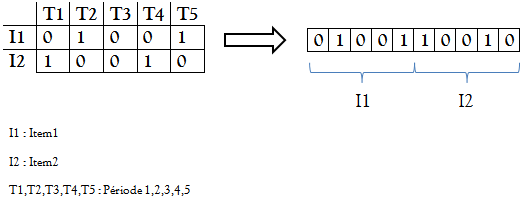
\includegraphics[scale=.5]{img/init_gene_repr.png}
			\caption{Représentation génétique initiale}
			\label{fig:init_gene_repr}
		\end{center}
	\end{figure}
	
	Autrement dit:
	\begin{center}
		$ch_{n} = \{(x_{1,1}),..., (x_{1,t+1}),..., ( x_{1,T}), (x_{j+1,1}),...,(x_{j+1, t+1}),..., (x_{j+1,T}),..., (x_{N,T})\}$ \\
	\end{center}
	\hspace*{.5cm} où $x_{N,T}$ est la variable booléenne qui indique la production ou non d'un article \emph{N} en période \emph{T}.  \\
	\\
	\hspace*{.5cm} Dans cette représentation, un chromosome est une chaîne de bits (0 et 1) qui indique la production ou non d'un article \emph{i} et de longueur \emph{nItems * nTimes} (où \emph{nItems} est le nombre d'articles et \emph{nTimes} est le nombre de périodes). Ainsi, l'article 1 est produit dans les périodes 2 et 5; et l'article 2 est produit dans les périodes 1 et 4. Le chromosome représenté ci-dessus est ainsi un plan de production qui satisfait aux contraintes du système de production spécifiques à cette instance du problème. Toutefois, au cours de notre étude, une seconde représentation nous est apparue plus cohérente et facilement manipulable. Cette représentation génétique est présentée à la figure \ref{fig:adopt_gene_repr} et étudiée par Mirshekarian et al.[ref].
	
	\begin{figure}[!h]
		\begin{center}
			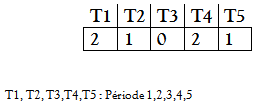
\includegraphics[scale=.5]{img/adopt_gene_repr.png}
			\caption{Représentation génétique adoptée}
			\label{fig:adopt_gene_repr}
		\end{center}
	\end{figure}
	
	Dans cette représentation, un chromosome est une suite d'entiers correspondant aux articles produits et de longueur \emph{nTimes}. La longueur réduite de ce chromosome réduit dans le même temps la complexité du parcours du chromosome lors des implémentations.
	\subsection{Initialisation}
	Le processus d'initialisation consiste à construire la population initiale; c'est à dire celle à partir de laquelle se feront les opérations de sélection, crossover ou encore mutation afin de la faire évoluer sur des générations. L'initialisation en algorithmes génétiques se fait de manière aléatoire dans l'optique de trouver des individus suffisamment différents capables de constituer une population diverse et ainsi que largement couvrir l'espace de recherche. \\
	\hspace*{.5cm} Une autre approche consiste à créer les individus devant composer la population initiale en se servant de stratégies de recherche déterministes et informés munis de fonctions d'évaluation suffisamment précises menant à des bonnes solutions. Notre approche a été de combiner les deux méthodes: utiliser une stratégie de recherche en l’occurrence le "Depth First Search" (DFS) dotée d'une fonction d'évaluation afin de déterminer lequel des fils à considérer; et utiliser une fonction de \emph{random} afin de rendre le parcours suffisamment aléatoire et conduisant à des individus différents. \\
	\hspace*{.5cm} L'algorithme d'initialisation mis en œuvre est ainsi détaillé comme suit: \\
	
	\begin{algorithm}[H]
 		\caption{Processus de génération de la population initiale}
 		\KwData{instance de PSP à traiter, taille de la population}
 		\BlankLine
 		\KwResult{Population initiale constituée}
 		\BlankLine
 	    $populationInitiale \gets tableau vide$  \\
 	    \BlankLine
 	    $item \gets random(1, nbItems)$ \\
 	    \BlankLine
 	    $listeDemandes \gets demandes(item)$ \\
 	    \BlankLine
 	    $demande \gets random(listeDemandes)$ \\
 	    \BlankLine
 	    $individu.satisfaireDemande(item, demande)$\\
 	    \BlankLine
 	    $root \gets creerNode(individu)$ \\
 	    \BlankLine
 	    $DFS(populationInitiale, individu, taillePopulation)$ \\
 	    \BlankLine
 	    \Return {$populationInitiale$}
	\end{algorithm}
	
	\vspace*{.5cm}
	La description de la stratégie de recherche DFS utilisée est effectuée comme suit: \\
	
	\begin{algorithm}[H]
		\caption{Description du Depth First Search utilisée}
 		\KwData{instance de PSP à traiter, taille de la population, root}
 		\BlankLine
 		\KwResult{Population initiale constituée}
		\BlankLine 		
 		\While{taille(populationInitiale) est inférieure à taillePopulation}{
 			\BlankLine
 			\If{individu est faisable}{
 				\BlankLine
 				$populationInitiale.ajouter(individu)$\\
 				\BlankLine
 				$individu \gets nouveauChromosome()$
 				\BlankLine
 			}
 			\BlankLine
 			//Générer les noeuds suivants \\
 			\BlankLine
 			\For { $ i \gets 1 $ \KwTo $ nbItems $ }{
 				\BlankLine
 				$item \gets random(1, nbItems)$ \\
 				\BlankLine
 				$listeDemandes \gets demandes(item)$ \\
 				\BlankLine
 				\For {demande in listeDemandes}{
 					\BlankLine
 					\For {period $\gets$ 0 \KwTo demande}{
 						\BlankLine
 						individu.insererItem(item, period)
 						\BlankLine
 						$node \gets creerNode(individu)$ \\
 						\BlankLine
 						$queue.inserer(individu)$
 						\BlankLine
 					}
 					\BlankLine
 				}
 				\BlankLine
 			}
 			\If{queue est vide}{
 				\BlankLine
 				arrêter \\
 				\BlankLine
 			}
 			\BlankLine
 			$node \gets queue.retirerDernier()$ 
 			\BlankLine	
	}
	\end{algorithm}	
	
	\subsection{Opérateurs génétiques}
		\subsubsection{Sélection}
		La sélection est le processus qui consiste à choisir dans la génération actuelle, les chromosomes ou individus qui seront reproduits afin de former la prochaine génération. Différentes méthodes de sélection existent. On distingue entre autres, la selection par tournoi et la sélection par "\emph{roulette wheel}". \\
		\hspace*{.5cm} Dans notre étude, nous choisissons de nous interesser à la plus connue et commune d'entre les méthodes de sélection: le \emph{"Roulette Wheel"}. Dans la sélection par "\emph{roulette wheel}", les individus se voient attribués une probabilité d'être sélectionnés. Cette probabilité est directement proportionnelle à leur fonction d'évaluation. Les individus sont donc choisis aléatoirement en se basant sur leur probabilité et se reproduisent en générant des individus "\emph{fils}". Ces "\emph{fils}" sont ainsi de nouvelles solutions au problème et forme une nouvelle population.
		\subsubsection{Croisement}
		
		Une fois les individus sélectionnés, intervient le croisement. Le croisement en un point a été choisi afin de reproduire ces individus. Cette forme de croisement reste une des plus simples et répandues. La figure \ref{fig:used_cross_over} présente une illustration du croisement appliqué à l'instance de PSP introduite à la page \pageref{ex:psp}. \\
		\begin{figure}[!h]
			\begin{center}
				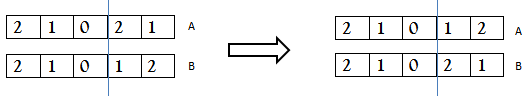
\includegraphics[scale=.5]{img/cross_over_fig.png}
				\caption{Illustration du croisement utilisé}
				\label{fig:used_cross_over}
			\end{center}
		\end{figure}
		
		\hspace*{.5cm} Le croisement se fait ainsi après la troisième période. Le croisement peut engendrer des individus qui, contrairement à la figure \ref{fig:used_cross_over}, ne respectent pas les contraintes de sytème en terme de \emph{shortage} ou de \emph{backlogging}. Il faut alors rendre ces individus à nouveau faisables avant de procéder à une quelconque mutation.
		  
	\subsubsection{Mutation}
	Après la sélection et le croisement, une nouvelle population d'individus est prête. Certains ont été copiés directement et d'autres se sont reproduits par croisement. Dans le but de s'assurer que les individus ne sont pas exactement les mêmes, une mutation est appliquée à chacun des individus "\emph{fils}". A chaque gène, on attribue une chance de muter. Dans le cas, où la mutation se produit, la valeur du gène muté change de période. Un visuel de la mutation est présenté à la figure \ref{fig:used_mutation}. La mutation est une élément vital de la garantie d'une diversité au sein de la population. 
	
	\begin{figure}[!h]
		\begin{center}
			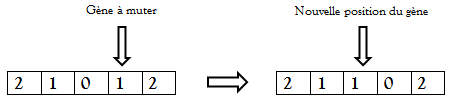
\includegraphics[scale=.5]{img/mutation_fig.png}
			\caption{Illustration de la méthode de mutation}
			\label{fig:used_mutation}
		\end{center}
	\end{figure}
	
	\subsection{Évaluation}
	L'évaluation dans notre étude, se réfère à la fonction objectif. Il s'agit de minimiser les coûts d'exploitation et de production. Deux types de coût sont à prendre en compte:
	\begin{itemize}
		\item[•] Les coûts de preparation ou \emph{setup} sont des coûts induis au moment d'un changement dans le configuration d'une ressource d'un type d'article à un autre. Il s'agit de perte potentielle de production durant le période de préparation, de force de travail additionnelle ou encore de ressources additionnelles brutes consommées durant la préparation.
		\item[•] Les coûts de stockage qui sont induis lors du conditionnement et d’entreposage.
	\end{itemize}
	
	\subsection{Terminaison}
	Deux moyens sont utilisés par lesquels les algorithmes génétiques se terminent. Habituellement, une limite est mise sur le nombre de générations après lesquelles le processus se termine. Avec certains problèmes, le processus de recherche se termine quand une solution particulière a été trouvée ou encore lorsque la plus haute valeur de "fitness" dans la population a atteint une valeur particulière. \\
	\hspace*{.5cm} Deux critères de terminaison sont utilisés dans notre étude afin de terminer une recherche. D'une part, la recherche se termine lorsque l'algorithme converge sur un individu considéré comme une solution optimale. D'autre part, une limite a été fixée sur le nombre de générations parcourues sans aucune amélioration de la valeur de "fitness" du meilleur individu de la population.
	
	\section{Algorithmes génétiques parallèles}	
	Les algorithmes génétiques sont des techniques de recherche qui ont été utilisées avec succès dans la résolution de problèmes dans différents disciplines. Cependant, la recherche permanente de performance dans l'exécution des algorithmes et le développement constant d'ordinateurs toujours plus performants et parallèles ont conduit à émergence d'un type d'algorithmes génétiques plus performants que les algorithmes génétiques standards. A propos des algorithmes génétiques parallèles, on distingue généralement trois classes : les "\emph{master-slave} parallel genetic algorithms", les "\emph{ coarsed-grained} parallel genetic algorithms" et les "\emph{fine-grained} parallel genetic algorithms". Les "master-slave parallel genetic algorithms" sont le type le plus simples d'algorithmes génétiques parallèles. Elles consistent essentiellement à distribuer l'évaluation de la population globale entre plusieurs processeurs. Le processeur qui conserve la population et exécute l'algorithme génétique est le maître et les processus qui évaluent la population sont les esclaves. La figure \ref{fig:master_slave_ga} montre un schéma de l'algorithme génétique parallèle "coarse-grained". Nous nous intéressons dans notre étude aux deux autres types, plus compliqués mais également plus intéressants dans leur fonctionnement et performances.
	
	\begin{figure}[!h]
		\begin{center}
			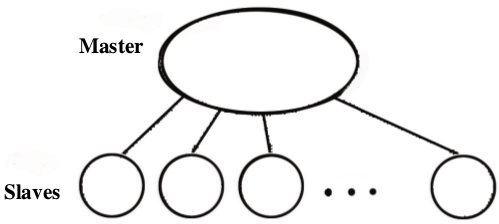
\includegraphics[scale=.3]{img/master_slave_ga.png}
			\caption{Schéma d'un algorithme génétique de type "master-slave"}
			\label{fig:master_slave_ga}
		\end{center}
	\end{figure}
	
	\newpage	
	
	\subsection{Algorithmes génétiques parallèles de type "\emph{coarse-grained}"}
	Les algorithmes génétiques de type "\emph{coarse-grained}" ou encore "\emph{modèle de l'île}" consiste en un ensemble de sous-populations qui échangent des individus de manière fréquente. Il s'agit probablement du type d'algorithmes génétiques le plus populaire bien qu'il nécessite de contrôler beaucoup de paramètres. La complète compréhension des effets de ces paramètres sur la qualité et la vitesse de recherche nous échappe encore. Cependant, Il a été démontré théoriquement que plus de sous-populations sont utilisées, leur taille peut être réduite sans sacrifier la qualité de la recherche. Vu que chaque processus s'exécute en parallèle, il en résulte une réduction du temps dédié aux calculs. Cependant, utiliser plus de sous-populations et donc de processus augmente la communication dans le système. Un compromis doit donc être effectué entre le temps de calculs et le temps de communication. L'implémentation des algorithmes génétiques parallèles soulève générale trois problématiques principalement sur la migration qui est l'échange d'individus entre processus. Il s'agit: de la fréquence de migration, du nombre d'individus à échanger, de la topologie des connections entre processus et de la méthode d'intégration des migrants.
	\subsubsection{Fréquence de migration}
	La migration affecte la qualité de la recherche et l'efficacité de l'algorithme en plusieurs points. Ainsi, de fréquentes migrations entraîne l'échange massif de potentiels bons matériels génétiques, mais il affecte aussi négativement la performance dans le mesure où les communications sont coûteuses. La même chose se produit dans les topologies densément connectées où chaque processus communique avec les autres. Le but ultime des algorithmes génétiques parallèles est de trouver de bonnes solutions assez rapidement. Il est donc nécessaire de trouver l'équilibre entre le coût de la migration et l'augmentation des chances de trouver de bonnes solutions. \\
	\hspace*{.5cm} Afin d'implémenter l'algorithme, nous avons donné à l'utilisateur la possibilité d'entrer l'intervalle de générations en les migrations. Cependant, le comportement par défaut de l'algorithme est de migrer uniquement lorsque la population a convergé complètement.  
	\subsubsection{Nombre de migrants}
	La migration envoie une nombre prédéterminé d'individus d'un processus à ces processus voisins logiques sur le graphe de communications. Ces individus ou "\emph{migrants}" seront ainsi intégrés dans le population des processus auxquels ils ont été envoyés. Il est possible de choisir les "migrants" de façon aléatoire ou alors de meilleurs individus de la population actuelle. La sélection aléatoire a l'avantage de disséminer plus diversité et les chances d'explorer de nouvelles régionsde l'espace de recherche peuvent être améliorer. La sélection des meilleurs individus peut aider à disséminer un matériel génétique qui a déjà été tester et qui serait doc intéressant. Dans la suite de notre étude, nous avons choisir d'échanger les meilleurs individus.
	\subsubsection{Topologie de connections}
	La topologie est également une importante partie des algorithmes génétiques de type \emph{"coarse-grained"}. En théorie, toute les topologies arbitraires peuvent être utilisées. Cependant, certains modèles sont fréquents. il s'agit : des topologies linéaires, des anneaux, des hypercubes. des densément connectés, des isolés. La topologie utilisé a été celle densément connectée présentée à la figure \ref{fig:topology_fig} 
	
	\begin{figure}[!h]
		\begin{center}
			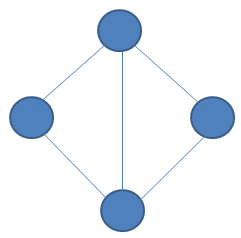
\includegraphics[scale=.3]{img/topology_fig.png}
			\caption{Topologie de connections utilisée}
			\label{fig:topology_fig}
		\end{center}
	\end{figure}
	
	\subsubsection{Méthode d'intégration des migrants}
 	Différentes alternatives existent pour incorporer les "\emph{migrants}". Deux d'entre elles sont récurrentes. Il s'agit: du remplacement aléatoire des individus de la population actuelle par les "\emph{migrants}" et du remplacement compétitif ou élitiste. Dans le remplacement aléatoire, les individus devant être remplacés sont désignés de manière aléatoire. Dans le remplacement compétitif, seules les individus avec les plus mauvais scores de "fitness" sont remplacés par les nouveaux arrivants.\\
 	\\
 	\hspace*{.5cm} Une fois, ces problématiques abordées, la question de l'implémentation rapide des algorithmes génétiques de type "\emph{coarse-grained}" revient. Une des réponses serait en effet de combiner ce type d'algorithmes génétiques avec un autre type, le "\emph{master-slave}" par exemple. On obtient alors un nouvelle classe d'algorithmes génétiques que sont les algorithmes génétiques hiérarchiques avec au niveau supérieur un algorithme génétique de type \emph{coarse-grained} et au niveau inférieur un algorithme génétique de type \emph{master-slave} comme le présente la figure \ref{fig:hierarchical_gene1_fig}. Il s'agit ainsi de cette combinaison que nous avons utilisée pour nos tests
 	
	\begin{figure}[!h]
		\begin{center}
			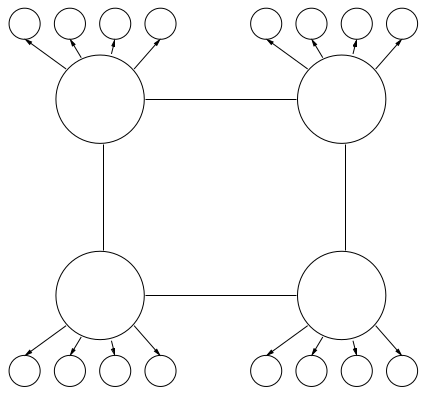
\includegraphics[scale=.3]{img/hierarchical_gene1_fig.png}
			\caption{Algorithmes génétiques hierarchiques avec au niveau supérieur un algorithme génétique de type \emph{coarse-grained} et au niveau inférieur un algorithme génétique de type \emph{master-slave}}
			\label{fig:hierarchical_gene1_fig}
		\end{center}
	\end{figure} 	
 	
	\subsection{Algorithmes génétiques parallèles de type "\emph{fine-grained}"}
	les algorithmes génétiques de type "\emph{fine-grained}" ont seulement une population, mais la structure spatiale limite les interactions entre les individus. Un individu ne peut compétir et se reproduire qu'avec ses individus voisins. Vu que les voisinages se chevauchent, les bonnes solutions peuvent ainsi se disséminer à travers la population entière. Le choix le plus important dans l'implémentation de ce type d'algorithmes génétiques sont : la topologie de connections.
	\subsubsection{Topologie de connections}
	Différentes topologies de connections sont valables. Il s'agit entre autres des grilles 2-D, des hypercubes, le torus, le cube. Il est cependant répandu de placer les individus dans un algorithme génétique de type "\emph{fine-grained}" dans une grille 2-Dimension. En effet, dans la plupart des ordinateurs massivement parallèles, les éléments de traitement et de calculs sont connectés en suivant cette topologie. La figure \ref{fig:fine_grained_fig} présente la topologie utilisée afin d'implémenter l'algorithme génétique de type \emph{"fine-grained"}.
	
	\subsubsection{Principe de fonctionnement}
	Le principe de fonctionnement des algorithmes génétiques de type "\emph{fine-grained}" est différent de ceux de type \emph{coarse-grained} et \emph{master-slave} est détaillé à l'algorithme \ref{alg:principe_fine_grained}. \\
	\\
	\begin{algorithm}[H]
		\label{alg:principe_fine_grained}
 		\caption{Principe des algorithmes génétiques parallèles de type "\emph{fine-grained}"}
 		\KwData{instance de PSP à traiter}
 		\BlankLine
 		\For{chaque nœud en parallèle}{
 		generer un individu de façon aléatoire
 		}
 		\BlankLine
 		\While{le critère de terminaison n'est pas satisfait}{
 			\For{chaque nœud en parallèle}{
 			evaluer le fitness de l'individu \\
 			obtenir la valeur de fitness des individus voisins \\
 			selectionner l'individu voisin dont la valeur de fitness est la plus grande \\
 			appliquer un croisement avec cet individu \\
 			muter l'individu qui en a résulté \\
 			}
 			Tester le critère de terminaison
 		}
	\end{algorithm}
	
	\begin{figure}[!h]
		\begin{center}
			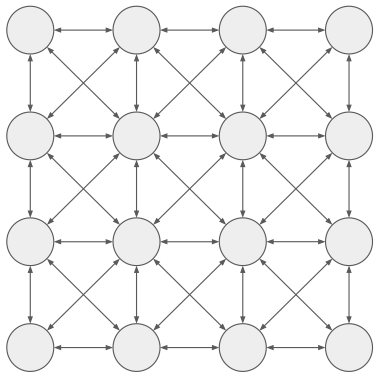
\includegraphics[scale=.3]{img/fine_grained_fig.png}
			\caption{Topologie utilisée en algorithme génétique de type "\emph{fine-grained}"}
			\label{fig:fine_grained_fig}
		\end{center}
	\end{figure} 
	
	\subsubsection{Algorithme hiérarchique entre \emph{fine-grained} et \emph{coarse-grained}}
	Des chercheurs ont combiné deux des méthodes de parallélisation produisant des algorithmes génétiques parallèles hiérarchiques. Certains de ces nouveaux algorithmes ajoutent un nouveau degré de complexité à des algorithmes déjà compliqués. On obtient alors des algorithmes génétiques parallèles hiérarchiques avec au niveau supérieur un algorithme génétique de type \emph{coarse-grained} et au niveau inférieur un algorithme génétique de type \emph{fine-grained} comme détaillé à la figure \ref{fig:hierar_fine_grained_fig}
	
	\begin{figure}[!h]
		\begin{center}
			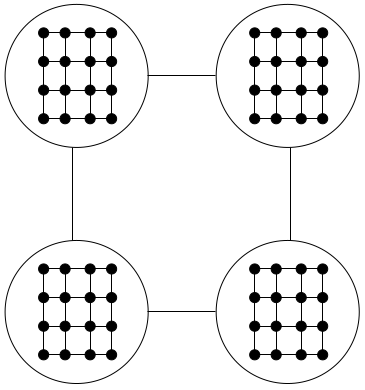
\includegraphics[scale=.3]{img/hierar_fine_grained_fig.png}
			\caption{Hiérarchie entre algorithmes génétiques parallèles de type \emph{fine-grained} et de type \emph{coarse-grained}}
			\label{fig:hierar_fine_grained_fig}
		\end{center}
	\end{figure} 
	\section{Autres implémentations}
	\subsection{Hybridation}
	L'hybridation consiste à combiner deux méthodes de recherche afin d'engendrer une nouvelle méthode de recherche dit \emph{hybride}. Les algorihmes génétiques facilite l'hybridation avec les autres techniques de recherche local afin d'obtenir la solution optimale. De façon basique, la recherche locale et les algorithmes génétiques sont complémentaires. Les algorithmes génétiques sont efficaces lorsqu'il s'agit de parcourir un espace de recherche global, dans le mesure où elles sont capables de rapidement des régions prometteuses. Cependant, elles prennent relativement beaucoup de temps à trouver des optimums dans ces régions. La recherche local est capable de trouver des optimums locaux avec une grande précision. \\
	\hspace*{.5cm} Dans notre étude, il s'est agi de mettre au point un algorithme de recherche qui est utilisé à chaque fois que l'algorithme génétique converge sur une solution optimale afin de parcourir l'espace de recherche immédiat à cette solution et ainsi améliorer cette solution optimale. 
	
	\subsection{Table de Hash}
	Dans le processus de réolution des problèmes à l'aides algorithmes génétiques, au fur et à mesure que les générations passent, la population évolue et la diversité au sein de cette dernière diminue amenant les mêmes chromosomes à être régulièrement réévalués. Dans les faits, l'effort de calculs dépensé à évaluer le "\emph{fitness}" dépasse celui dépensé sur les opérateurs génétiques. En utilisant une table de hash afin de stocker les chromosomes récemment évalués, une amélioration significative des performances peut être constatée. Nous avons donc utilisé un dictionnaire ou tableau associatif afin de stocker ces derniers.
	
	\section*{Conclusion}
	\addcontentsline{toc}{section}{Conclusion}
	
	\newpage
	
	\part{Expérimentations et Analyse des résultats}
	\setcounter{section}{0}
	%\newpage
		\section*{Introduction}
		\addcontentsline{toc}{section}{Introduction}
		L'expérimentation lors d'une étude est une étape importante du travail de recherche. Il s'agit le plus souvent donc de tester les théories émises et d'analyser les résultats obtenus de tests afin de valider nos approches de solution du problème énoncées. Dans cette partie, nous présentons d'abord l'environnement de test, les instances utilisées. Ensuite, nous expérimentons nos solutions et à partir des résultats obtenus, nous comparons nos approches heuristiques basées sur les algorithmes génétiques à celles déjà appliquées à ce problème.
		
		\section{Environnement de test} 
		
		\subsection{Matériel}
		Pour l'implémentation de nos tests, nous avons travaillé sur un ordinateur présentant les caractéristiques suivantes :\\
		\begin{itemize}
			\item[•] Système d'exploitation: Linux Ubuntu 16.04 LTS; \\
			\item[•] Processeur: Intel®  Core \up{\textsc{TM}} i7 CPU L 640 @ 2.13GHz x 4; \\
			\item[•] Mémoire: 3,7 Gio;\\
			\item[•] Type du système d'exploitation: 64 bits.\\
		\end{itemize}
		\subsection{Langage de programmation}
		Le langage de programmation utilisée afin de d'implémenter notre solution est le langage \emph{Python} dans sa version Python 3.5. \emph{Python} est un puissant langage de programmation interprété qui apparaît de plus en plus comme une alternative crédible et intéressante dans le domaine de l'intelligence artificielle, tant il présente des qualités quant à sa robustesse, sa rapidité, sa portabilité, sa facilité de prise en main, sa rigueur et sa caractéristique de langage Open source.  
		
		\subsection{Données de test}
		
		Deux ensembles d'instances ont été utilisés dans notre étude afin de tester nos deux solutions. Il s'agit d'une part de celles disponibles dans la bibliothèque \emph{CSPlib} à https://bitbucket.org/ratheilesse/cp4ppet proposées par Houndji et al. (2014). D'autres part, Ceschia et al dans leur application du recuit simulé au PSP ont mis au point un générateur paramétré. Leur générateur reçoit entre autres comme entrées, le nombre d'articles, le nombre de périodes et produit en sortie une instance aléatoire à l'aide de ces paramètres. Ces instances sont disponibles à http://opthub.uniud.it.
		
		\begin{description}
			\item[CSPlib] 
			\item[Opthub]
		\end{description}
		
		\section{Résultats expérimentaux du Fine-grained Parallel Genetic Algorithm}
		\section{Résultats expérimentaux du Coarse-grained Parallel Genetic Algorithm}
		\section{Analyse comparative des résultats}
		\section*{Conclusion}
		\addcontentsline{toc}{section}{Conclusion}
		
	\newpage
		
	\part*{Conclusion et Perspectives}
	\addcontentsline{toc}{part}{Conclusion et Perspectives}
	
	\newpage
	
	\part*{Bibliographie}
	\addcontentsline{toc}{part}{Bibliographie}
	
	\newpage
	
	\appendix
	\part*{Annexes}
	\addcontentsline{toc}{part}{Annexes}
	\section{Extension au problème de planification de production avec plusieurs machines}
		\subsection{Description du problème}
		On s’intéresse ici à un problème de planification de production avec plu-
sieurs machines de capacités finies et constantes. Il y a plusieurs articles à
produire sur un horizon de planification discret et fini. La demande est statique et déterministe et il n’y a pas de shortage. La fonction objectif comprend
les coûts de :
		\begin{itemize}
			\item[•] \emph{setup}: lorsqu’on prépare une machine pour la production d’un article à une période donnée. Ce coût est induit une seule fois
à une période donnée même si on produit plusieurs fois le même article sur la machine ;
			\item[•] \emph{inventory} : lorsqu'on conserve en stocks des articles afin de pouvoir satisfaire les demandes.
		\end{itemize}
		\subsection{Modèle et formulation}
		\subsection{Notre solution}
		\subsection{Expérimentations et Analyse des résultats}
		
	\section{Conception et Structure du programme}

\end{document}